% ============================================================
% IEEE PAPER: Deteksi DDoS Berbasis XGBoost dan Information Gain
% Template: IEEEtran (conference, A4)
% Compile: pdflatex > bibtex > pdflatex > pdflatex
% ============================================================
\documentclass[conference,a4paper]{IEEEtran}

% ── PACKAGES ────────────────────────────────────────────────
\usepackage[utf8]{inputenc}
\usepackage[T1]{fontenc}
\usepackage{amsmath,amssymb,amsfonts}
\usepackage{algorithmic}
\usepackage{algorithm}
\usepackage{graphicx}
\usepackage{textcomp}
\usepackage{xcolor}
\usepackage{booktabs}
\usepackage{multirow}
\usepackage{array}
\usepackage{url}
\usepackage{hyperref}
\usepackage{cite}
\usepackage{balance}
\usepackage[indonesian]{babel}

\hypersetup{
    colorlinks=true,
    linkcolor=blue,
    citecolor=blue,
    urlcolor=blue
}

\def\BibTeX{{\rm B\kern-.05em{\sc i\kern-.025em b}\kern-.08em
    T\kern-.1667em\lower.7ex\hbox{E}\kern-.125emX}}

% ============================================================
\begin{document}

% ── JUDUL ────────────────────────────────────────────────────
\title{Pengembangan Perangkat Lunak Deteksi dan Forensik Jaringan DDoS Berbasis XGBoost dan Information Gain}

\author{
  \IEEEauthorblockN{%
    Falito Eriano Nainggolan,\,
    Dimas Surya Pratama,\,
    Gita Olivia Silaban%
  }
  \IEEEauthorblockA{%
    Program Studi Rekayasa Keamanan Siber\\
    Politeknik Siber dan Sandi Negara, Bogor, Indonesia\\
    Email: falito.eriano@poltekssn.ac.id, dimas.surya@poltekssn.ac.id, gita.olivia@poltekssn.ac.id
  }
}

\maketitle
\vspace{-0.35cm}

% ── ABSTRAK ──────────────────────────────────────────────────
\begin{abstract}
Serangan \textit{Distributed Denial of Service} (DDoS) merupakan salah satu
ancaman utama bagi keamanan jaringan di lingkungan kampus. Kampus biasanya
memiliki jaringan yang terbuka karena banyak mahasiswa dan staf yang menghubungkan
perangkat pribadi mereka secara bebas. Sayangnya, sistem pendeteksi dan analisis forensik serangan DDoS
yang ringan, akurat, dan mudah digunakan langsung di kampus masih sangat terbatas.
Oleh karena itu, dalam penelitian ini kami mengembangkan DDoShield, sebuah perangkat lunak
web untuk deteksi dan forensik jaringan DDoS menggunakan algoritma XGBoost dan seleksi fitur
\textit{Information Gain} (IG). Eksperimen kami lakukan menggunakan dataset
standar CIC-IDS2017 (225.745 sampel data dan 78 fitur). Kami menguji performa model
dengan variasi jumlah fitur $K = \{5, 10, 15, 20, 30, \text{all}\}$ dan membandingkan
XGBoost dengan algoritma \textit{Random Forest} menggunakan uji statistik McNemar.
Hasil eksperimen menunjukkan bahwa XGBoost dengan $K=30$ fitur terbaik mampu mencapai
\textit{F1-Score} sebesar \textbf{99,9977\%} dan nilai AUC-ROC sebesar \textbf{1,0000}.
Dari 45.149 data uji, model kami hanya salah menebak \textbf{1 sampel} saja.
Seleksi fitur IG berhasil memangkas waktu pelatihan sebesar 52,7\% (dari 9,38\,s menjadi 4,44\,s)
tanpa mengurangi akurasi. Selanjutnya, perbandingan antara XGBoost dan \textit{Random Forest}
pada K=30 menggunakan uji statistik McNemar ($p=0{,}4795$) menunjukkan bahwa akurasi keduanya
tidak berbeda secara signifikan, namun XGBoost jauh lebih unggul dalam kecepatan komputasi:
waktu pelatihan 6,9$\times$ lebih cepat dan waktu deteksi per flow
1,6$\times$ lebih cepat (0,0051\,ms vs.\ 0,0084\,ms/flow). Hasil ini membuktikan bahwa
kombinasi XGBoost dan seleksi fitur IG sangat cocok dan efisien untuk analisis forensik dan deteksi DDoS di
jaringan kampus yang memiliki keterbatasan spesifikasi komputer server.
\end{abstract}

\begin{IEEEkeywords}
deteksi dan forensik DDoS; XGBoost; \textit{information gain}; seleksi fitur; CIC-IDS2017;
keamanan jaringan kampus; \textit{intrusion detection system}; \textit{machine
learning}
\end{IEEEkeywords}

% ============================================================
\section{Pendahuluan}
% ============================================================

Serangan \textit{Distributed Denial of Service} (DDoS) merupakan salah satu masalah
keamanan komputer yang paling sering terjadi dan merugikan di dunia. Berdasarkan laporan
keamanan dari NETSCOUT, jumlah serangan DDoS terus meningkat setiap tahunnya~\cite{ref_netscout2023}.
Laporan dari Cloudflare juga menyebutkan bahwa serangan DDoS berbasis web (HTTP) naik
sebesar 65\% dibanding tahun sebelumnya~\cite{ref_cloudflare2023}. Serangan ini bekerja dengan
cara membanjiri komputer server menggunakan trafik palsu dari banyak komputer penyerang, sehingga
pengguna asli kesulitan atau bahkan tidak bisa mengakses layanan web tersebut.

Di lingkungan kampus, masalah keamanan ini menjadi tantangan tersendiri. Jaringan kampus
biasanya dirancang terbuka untuk memudahkan mahasiswa, dosen, dan staf mengakses internet
atau layanan akademik. Selain itu, adanya kebijakan \textit{Bring Your Own Device} (BYOD)
membuat siapa saja bisa menghubungkan laptop atau ponsel pribadi mereka ke jaringan kampus~\cite{ref_byod}.
Hal ini membuat jaringan kampus menjadi sasaran yang mudah diserang malware. Di sisi lain,
tim TI di kampus sering kali memiliki keterbatasan jumlah staf dan spesifikasi perangkat keras
untuk menangani serangan DDoS yang mendadak~\cite{ref_campus_sec}.

Selama ini, sistem pendeteksi penyusupan (\textit{Intrusion Detection System} atau IDS)
yang digunakan masih memiliki beberapa kelemahan. Pertama, IDS tradisional yang memakai sistem
pencocokan pola (\textit{signature-based}) tidak bisa mendeteksi jenis serangan DDoS baru yang belum
terdaftar di database mereka (serangan \textit{zero-day})~\cite{ref_ring2019}. Kedua, banyak metode
\textit{machine learning} yang diusulkan dalam penelitian sebelumnya langsung memakai semua fitur data
(bisa sampai 78 fitur) tanpa mencari tahu fitur mana yang sebenarnya paling penting~\cite{ref_kasongo2020,ref_ullah2020}.
Hal ini membuat pemrosesan data menjadi lambat dan berat. Ketiga, jarang ada penelitian akademis
yang membuat aplikasinya sampai jadi dan bisa langsung dicoba secara nyata oleh pengguna~\cite{ref_abdulganiyu2023}.

Untuk mengatasi masalah tersebut, dalam penelitian ini kami bertujuan untuk:
(1)~mencari tahu berapa jumlah fitur terbaik (dari variasi $K = \{5, 10, 15, 20, 30, \text{all}\}$)
menggunakan metode seleksi fitur \textit{Information Gain}; (2)~membandingkan performa algoritma
XGBoost dan \textit{Random Forest} pada jumlah fitur terbaik tersebut; (3)~membuat aplikasi web
DDoShield untuk deteksi dan forensik jaringan yang bisa menganalisis file trafik \texttt{.pcap} secara langsung; dan (4)~menguji
performa aplikasi tersebut secara riil.

Penelitian ini diharapkan dapat memberikan kontribusi berupa: (1)~analisis sistematis pemilihan
fitur terbaik untuk deteksi dan forensik DDoS; (2)~perbandingan performa XGBoost dan \textit{Random Forest} yang
diperkuat dengan uji statistik McNemar; (3)~\textit{software} deteksi dan forensik jaringan (DDoShield) yang siap pakai;
dan (4)~hasil pengukuran kinerja sistem yang nyata pada lingkungan lokal.

Sisa paper ini disusun sebagai berikut: Seksi~\ref{sec:tinjpus} menjelaskan tinjauan pustaka;
Seksi~\ref{sec:metode} membahas metode penelitian kami; Seksi~\ref{sec:hasil} memaparkan hasil
eksperimen dan analisis; Seksi~\ref{sec:diskusi} membahas temuan penelitian; dan Seksi~\ref{sec:kesimpulan}
menyimpulkan hasil penelitian kami.

% ============================================================
\section{Tinjauan Pustaka}
\label{sec:tinjpus}
% ============================================================

\subsection{Karakteristik Serangan DDoS pada Jaringan Kampus}

Serangan DDoS bekerja dengan cara menghabiskan kapasitas \textit{bandwidth} jaringan atau membebani
sumber daya komputer server target menggunakan trafik yang sangat besar~\cite{ref_chandola2009}. Trafik
ini biasanya dikirim secara bersamaan oleh banyak komputer yang telah terinfeksi \textit{malware}
(biasa disebut \textit{botnet})~\cite{ref_ring2019}. Secara umum, serangan DDoS dibagi menjadi tiga
kelompok utama: (1)~\textit{volumetric attacks} yang bertujuan menghabiskan \textit{bandwidth} internet;
(2)~\textit{protocol attacks} yang memanfaatkan celah pada aturan protokol komunikasi data; dan
(3)~\textit{application layer attacks} yang menyerang langsung aplikasi atau layanan web server yang sedang berjalan.

\subsection{Evolusi Sistem Deteksi Intrusi}

Untuk mendeteksi serangan ini, sistem pendeteksi penyusupan (IDS) berbasis \textit{machine learning} (ML)
menawarkan solusi yang lebih pintar. Dibandingkan dengan metode biasa yang kaku, metode ML bisa mengenali
tanda-tanda aneh pada trafik jaringan secara otomatis tanpa perlu memiliki daftar tanda serangan (\textit{signature})
terlebih dahulu~\cite{ref_chandola2009}. Beberapa algoritma ML yang sering digunakan untuk tugas ini
antara lain \textit{Decision Tree}~\cite{ref_dt_ids}, \textit{Random Forest}~\cite{ref_ullah2020},
\textit{Convolutional Neural Network} (CNN)~\cite{ref_cnn_ids}, \textit{Long Short-Term Memory} (LSTM)~\cite{ref_lstm_ids},
dan XGBoost~\cite{ref_thakkar2020}.

\subsection{XGBoost untuk Deteksi Intrusi}

XGBoost (\textit{eXtreme Gradient Boosting}) adalah algoritma pembelajaran mesin berbasis pohon keputusan (\textit{decision tree}) yang sangat populer karena kecepatan dan akurasinya yang tinggi~\cite{ref_xgboost2016}. Algoritma ini bekerja dengan cara membangun banyak pohon keputusan secara berurutan, di mana setiap pohon baru bertugas memperbaiki kesalahan tebakan dari pohon-pohon sebelumnya. Keunggulan utama XGBoost adalah kemampuannya untuk mencegah model agar tidak terlalu menghafal data secara berlebihan (\textit{overfitting}) menggunakan fungsi pembatas (\textit{regularization}) bawaan, sehingga performa model tetap stabil saat menguji data baru~\cite{ref_xgboost2016}.

\subsection{Information Gain untuk Seleksi Fitur}

\textit{Information Gain} (IG) adalah metode yang kami gunakan untuk mengukur seberapa penting atau berharganya informasi dari suatu fitur dalam menentukan apakah suatu lalu lintas jaringan merupakan serangan DDoS atau trafik normal (\textit{BENIGN})~\cite{ref_shannon1948}. Konsep dasar IG berfokus pada tingkat ketidakpastian data (\textit{entropy}). Fitur yang memiliki nilai IG tinggi berarti mengandung informasi yang sangat kuat untuk membedakan antara trafik normal dan serangan. Sebaliknya, fitur dengan nilai IG mendekati nol dianggap tidak penting. Dengan menggunakan metode seleksi fitur berbasis IG ini, kami dapat membuang fitur-fitur yang tidak relevan sehingga model bisa bekerja jauh lebih cepat dan ringan saat dijalankan di server~\cite{ref_guyon2003}.

\subsection{Dataset CIC-IDS2017}

Dalam penelitian ini, kami menggunakan dataset CIC-IDS2017 yang dibuat oleh \textit{Canadian Institute for
Cybersecurity} (CIC)~\cite{ref_sharafaldin2018}. Dataset ini berisi rekaman trafik jaringan normal dan berbagai
jenis serangan selama lima hari kerja. Rekaman trafik tersebut kemudian diproses menggunakan program CICFlowMeter
sehingga menghasilkan 78 fitur berbasis flow. Kami menggunakan file data khusus bernama
\texttt{\small Friday-\allowbreak WorkingHours-\allowbreak Afternoon-\allowbreak DDos.\allowbreak pcap\_ISCX.csv} yang berisi 225.745 baris data, dengan rincian
128.027 data serangan DDoS (56,7\%) dan 97.718 data normal (BENIGN) (43,3\%).

\begin{table}[htbp]
\vspace{-0.2cm}
\caption{Perbandingan Penelitian Terkait}
\label{tab:related_work}
\centering
\small
\begin{tabular}{p{1.0cm}p{1.5cm}p{2.2cm}p{1.0cm}p{0.8cm}}
\toprule
\textbf{Ref.} & \textbf{Dataset} & \textbf{Algoritma} &
\textbf{Acc.} & \textbf{K} \\
\midrule
\cite{ref_thakkar2020}     & CIC-IDS & XGBoost+Corr  & 99,5\% & all \\
\cite{ref_kasongo2020}     & UNSW    & XGBoost+IG    & 99,2\% & 10 \\
\cite{ref_ullah2020}       & CIC-IDS & RF            & 98,7\% & 20 \\
\cite{ref_cnn_ids}         & CIC-IDS & CNN           & 99,1\% & all \\
\cite{ref_lstm_ids}        & CICIDS  & LSTM          & 98,3\% & all \\
\cite{ref_abdulganiyu2023} & Review  & Multi-algo    & --     & -- \\
\textbf{Kami}              & CIC-IDS & \textbf{XGB+IG} & \textbf{$\approx$100\%} & \textbf{30} \\
\bottomrule
\end{tabular}
\end{table}

% ============================================================
\section{Metodologi}
\label{sec:metode}
% ============================================================

\subsection{Alur Penelitian}

Penelitian yang kami lakukan terdiri dari tujuh tahapan, yaitu: (1)~menyiapkan dataset CIC-IDS2017;
(2)~membersihkan data (\textit{preprocessing}); (3)~menghitung skor IG dan memilih fitur terbaik;
(4)~mencari parameter model XGBoost yang paling cocok (\textit{hyperparameter tuning});
(5)~menguji variasi jumlah fitur K; (6)~membandingkan performa XGBoost dengan \textit{Random Forest};
dan (7)~membuat serta menguji aplikasi web DDoShield.

\subsection{Preprocessing Data}

Sebelum data digunakan untuk melatih model, kami melakukan beberapa langkah pembersihan data:
(1)~hanya mengambil baris data yang berlabel DDoS dan BENIGN; (2)~mengubah nilai tak hingga ($\pm\infty$)
menjadi data kosong (NaN); (3)~menghapus fitur yang memiliki lebih dari 50\% data kosong;
(4)~mengisi data kosong yang tersisa dengan nilai tengah (\textit{median}) karena statistik ini lebih tangguh (\textit{robust}) terhadap anomali ekstrem yang sering memicu \textit{Infinity} pada rekaman \textit{capture}; dan
(5)~menyamakan skala data (\textit{normalisasi}) menggunakan \texttt{StandardScaler} agar rentang nilainya
seragam. Setelah dibersihkan, data dibagi menjadi 80\% untuk data latih (\textit{training}) dan 20\% untuk
data uji (\textit{testing}) secara acak menggunakan \textit{stratified random sampling} untuk menjaga keseimbangan kelas. Kami menyadari bahwa pembagian acak pada data \textit{time-series} rentan terhadap bias \textit{data leakage}. Namun, protokol ini tetap kami pertahankan agar performa model dapat dikomparasikan secara \textit{apple-to-apple} dengan \textit{baseline} penelitian terdahulu yang jamak menggunakan metode serupa pada CIC-IDS2017.

\subsection{Seleksi Fitur Information Gain}

Kami menghitung nilai IG untuk semua 78 fitur menggunakan fungsi \texttt{mutual\_info\_classif} dari
pustaka Scikit-learn di Python (yang secara matematis menghitung \textit{Mutual Information}, ekuivalen dengan \textit{Information Gain} pada target diskrit). Setelah mendapatkan skor kepentingan masing-masing fitur, kami menggunakan
fungsi \texttt{SelectKBest} untuk memilih fitur-fitur terbaik dengan variasi jumlah
$K = \{5, 10, 15, 20, 30, \text{all}\}$. Secara keseluruhan, proses komputasi mulai dari \textit{preprocessing}, pelatihan, hingga inferensi dijalankan pada komputer lokal berspesifikasi Intel Core i7 dengan memori RAM 16GB dan sistem operasi Windows.

\subsection{Konfigurasi Model}

Untuk mendapatkan model XGBoost yang optimal, kami melakukan pencarian parameter terbaik menggunakan metode
\texttt{RandomizedSearchCV} dengan 20 kali percobaan dan 5-fold \textit{cross-validation} (menggunakan metrik
\textit{F1-Score} sebagai patokan penilaian). Parameter terbaik yang kami dapatkan adalah: \texttt{n\_estimators}=300
(jumlah pohon), \texttt{max\_depth}=4 (kedalaman pohon), \texttt{learning\_rate}=0,2, \texttt{subsample}=0,7,
\texttt{colsample\_bytree}=0,8, dan \texttt{scale\_pos\_weight}=0,7633. Sementara itu, untuk model pembanding
\textit{Random Forest}, kami menggunakan konfigurasi standar: \texttt{n\_estimators}=200,
\texttt{max\_features}=\texttt{sqrt}, dan \texttt{class\_weight}=\texttt{balanced}.

Metrik evaluasi yang kami gunakan untuk mengukur kinerja model ini meliputi:
\begin{itemize}
  \item \textbf{Akurasi (Accuracy)}: Menghitung persentase tebakan benar dari keseluruhan data uji.
  \item \textbf{Presisi (Precision)}: Mengukur seberapa tepat model mendeteksi DDoS tanpa salah menuduh data normal (meminimalkan \textit{False Positive}).
  \item \textbf{Recall}: Mengukur kemampuan model dalam menangkap semua serangan DDoS yang terjadi tanpa ada yang lolos (meminimalkan \textit{False Negative}).
  \item \textbf{F1-Score}: Nilai rata-rata seimbang dari Presisi dan Recall, yang menjadi acuan utama kami karena metrik ini memberikan evaluasi yang lebih komprehensif dibandingkan akurasi saja.
  \item \textbf{False Positive Rate (FPR)}: Persentase data normal yang tidak sengaja terdeteksi sebagai serangan DDoS oleh model.
\end{itemize}

\subsection{Arsitektur DDoShield dan Alur Kode Program}

Aplikasi DDoShield dirancang dengan arsitektur modular tiga lapis (\textit{presentation}, \textit{application}, \textit{data}) menggunakan Flask di Python. Aplikasi ini mendukung dua mode operasional: (1)~Analisis Luring (mengunggah berkas capture \texttt{.pcap} atau \texttt{.csv}), dan (2)~Live Sniffing (mengendus paket secara langsung dari antarmuka jaringan lokal secara real-time selama durasi tertentu menggunakan modul pengendus Scapy). Alur logika pemrograman di backend (\texttt{app.py}) dirancang secara transparan untuk menjamin validitas dan reproduksibilitas deteksi:


\begin{enumerate}
  \item \textbf{Ekstraksi Aliran (Flow Extraction)}: Berkas \texttt{.pcap} yang diunggah dibaca menggunakan pustaka Scapy. Paket data dikelompokkan menjadi aliran (\textit{flow}) berdasarkan kombinasi 5-tuple: IP sumber, IP tujuan, port sumber, port tujuan, dan protokol. Waktu kedatangan paket (\texttt{pkt.time}) dikonversi ke tipe data \textit{float} untuk menghindari kesalahan komputasi pembagian pada pustaka NumPy saat menghitung statistik durasi aliran dan jeda kedatangan paket (\textit{Flow IAT}).
  \item \textbf{Sistem Deteksi Hibrida (Hybrid Engine)}: Sebelum melewati klasifikasi mesin pembelajar, aliran data disaring terlebih dahulu oleh modul heuristik (\textit{Heuristics Engine}) untuk mengatasi masalah keterbatasan data latih (\textit{generalization gap}). Aturan heuristik dirancang berbasis batas ambang (\textit{threshold}) volume paket pada port layanan spesifik yang sering disalahgunakan untuk serangan amplifikasi, yaitu DNS (Port 53), NTP (Port 123), SSDP (Port 1900), dan Memcached (Port 11211). Jika sebuah aliran melebihi batas 50 paket pada port tersebut, aliran tersebut langsung diklasifikasikan sebagai serangan DDoS (misalnya, \textit{DDoS (DNS Amp)}).
  \item \textbf{Pipeline Machine Learning Terarah}: Aliran data yang tidak memicu aturan heuristik akan diekstraksi ke dalam 78 fitur numerik standar CICFlowMeter. Data ini kemudian diumpankan ke dalam pipeline pemrosesan Scikit-Learn:
  \begin{itemize}
    \item \textit{SimpleImputer} (\texttt{imputer.pkl}): Mengisi nilai kosong/NaN dengan nilai median kolom data latih.
    \item \textit{StandardScaler} (\texttt{scaler.pkl}): Menormalisasi skala data numerik.
    \item \textit{SelectKBest} (\texttt{selector\_kopt.pkl}): Memilih hanya 30 fitur optimal yang memiliki skor \textit{Information Gain} tertinggi.
    \item \textit{XGBoost Classifier} (\texttt{xgb\_model\_kopt.pkl}): Menentukan hasil klasifikasi akhir (DDoS atau BENIGN).
  \end{itemize}
\end{enumerate}

\begin{algorithm}[htbp]
\caption{Skema Deteksi Hibrida DDoShield}
\label{alg:hibrida}
\begin{algorithmic}[1]
\scriptsize
\REQUIRE Berkas Capture Jaringan $P$ (\texttt{.pcap} atau \texttt{.csv})
\ENSURE Hasil Deteksi Aliran $D$ (BENIGN atau DDoS)
\STATE $F \leftarrow \text{EkstraksiFlow}(P)$ \COMMENT{Mengelompokkan paket berdasarkan 5-tuple}
\FOR{setiap aliran $f \in F$}
    \STATE $\text{is\_heur}, \text{label} \leftarrow \text{PeriksaAturanHeuristik}(f)$
    \IF{$\text{is\_heur} = \text{True}$}
        \STATE $D(f) \leftarrow \text{label}$ \COMMENT{DNS/NTP/SSDP/Memcached Amplification}
    \ELSE
        \STATE $f_{imputed} \leftarrow \text{ImputasiNilaiTengah}(f)$ \COMMENT{SimpleImputer}
        \STATE $f_{scaled} \leftarrow \text{StandardisasiSkala}(f_{imputed})$ \COMMENT{StandardScaler}
        \STATE $f_{K30} \leftarrow \text{SeleksiFitur}(f_{scaled}, K=30)$ \COMMENT{SelectKBest}
        \STATE $\text{skor\_pred} \leftarrow \text{XGBoostClassifier}(f_{K30})$
        \IF{$\text{skor\_pred} = 1$}
            \STATE $D(f) \leftarrow \text{"DDoS (XGBoost)"}$
        \ELSE
            \STATE $D(f) \leftarrow \text{"BENIGN"}$
        \ENDIF
    \ENDIF
\ENDFOR
\RETURN $D$
\end{algorithmic}
\end{algorithm}


Seluruh model dan objek pipeline disimpan dalam format berkas serialisasi \texttt{.pkl} pada direktori lokal aplikasi agar dapat dijalankan secara luring (\textit{offline}) tanpa memerlukan koneksi internet, guna menjaga privasi data lalu lintas jaringan kampus.

Sebagai instrumen investigasi, kami mendefinisikan kapabilitas transparansi (\textit{Explainable AI}) ini sebagai bentuk \textbf{Forensik Berbasis Aliran (\textit{Flow-based Forensics})}. DDoShield membedah jejak logis serangan menggunakan nilai kontribusi lokal berbasis algoritma \textit{TreeSHAP} dari XGBoost~\cite{ref_interp}. Setiap kali pengguna mengklik baris aliran mencurigakan pada dasbor web, sistem memanggil REST API untuk menghitung dan memvisualisasikan 5 fitur dominan yang melatarbelakangi vonis DDoS (misalnya anomali pada \textit{Fwd Packet Length}). Analisis ini memberikan konteks forensik instan kepada administrator untuk mengidentifikasi anatomi serangan tanpa perlu mengisolasi \textit{payload} paket secara manual (\textit{Deep Packet Inspection}).




% ============================================================
\section{Hasil dan Analisis}
\label{sec:hasil}
% ============================================================

\subsection{Performa XGBoost per Variasi K}

Tabel~\ref{tab:xgb_k} menunjukkan hasil evaluasi performa klasifikasi untuk model XGBoost murni pada berbagai jumlah fitur K. Pengujian ini dilakukan secara spesifik pada modul \textit{Machine Learning} (tanpa pelibatan saringan \textit{Heuristic Engine}) menggunakan pembagian data latih-uji 80/20 untuk mengukur kapabilitas algoritmanya secara terisolasi.

\begin{table*}[t]
\caption{Performa XGBoost per Variasi K pada Dataset CIC-IDS2017}
\label{tab:xgb_k}
\centering
\footnotesize
\begin{tabular}{cccccccc}
\toprule
\textbf{K} & \textbf{Accuracy (\%)} & \textbf{Prec. (\%)} & \textbf{Recall (\%)} &
\textbf{F1-Score (\%)} & \textbf{AUC-ROC} & \textbf{Training (s)} & \textbf{Infer. (ms/flow)} \\
\midrule
5         & 99,88 & $\geq$99,8 & $\geq$99,8 & 99,89 & 0,9999 & 5,54 & 0,003 \\
10        & 99,94 & $\geq$99,9 & $\geq$99,9 & 99,95 & 1,0000 & 3,41 & 0,002 \\
15        & 99,96 & $\geq$99,9 & $\geq$99,9 & 99,96 & 1,0000 & 3,59 & 0,002 \\
20        & 99,98 & $\geq$99,9 & $\geq$99,9 & 99,98 & 1,0000 & 3,88 & 0,003 \\
\textbf{30} $\star$ & \textbf{99,9978} & \textbf{100,00} & \textbf{99,9961} & \textbf{99,9977} & \textbf{1,0000} & \textbf{4,44} & \textbf{0,005} \\
all (78)  & 99,9978 & 100,00 & 99,9961 & 99,9977 & 1,0000 & 9,38 & 0,005 \\
\bottomrule
\multicolumn{8}{l}{\small $\star$ = K optimal; Prec./Recall macro-average.}
\end{tabular}
\end{table*}

Pada K=5, model sudah menghasilkan \textit{F1-Score} sebesar 99,89\%, yang mana sudah sangat bagus tetapi
merupakan yang terendah dibanding pilihan K lainnya, sebagaimana ditunjukkan pada Gambar~\ref{fig:f1k}. Akurasi terus naik seiring bertambahnya fitur, hingga
mencapai performa tertinggi pada K=30 (\textit{F1-Score} 100,00\% atau tepatnya 99,9977\%). Menariknya,
menggunakan K=30 fitur memberikan akurasi yang sama persis dengan menggunakan semua 78 fitur. Hal ini
membuktikan bahwa 48 fitur lainnya tidak terlalu dibutuhkan karena informasinya tumpang tindih (\textit{redundan})
dengan fitur yang sudah terpilih~\cite{ref_kasongo2020}.

Berdasarkan hasil IG pada Gambar~\ref{fig:ig}, fitur-fitur yang paling membantu model dalam mendeteksi DDoS
adalah \textit{Total Length of Fwd Packets} (IG=0,652), \textit{Subflow Fwd Bytes} (IG=0,652),
\textit{Average Packet Size} (IG=0,563), dan \textit{Destination Port} (IG=0,542). Fitur-fitur ini menunjukkan
ukuran dan jumlah paket data yang dikirim, yang memang sangat mencerminkan pola serangan DDoS jenis \textit{flooding}
(membanjiri trafik)~\cite{ref_sharafaldin2018}.

\begin{figure}[htbp]
  \centering
  \begin{minipage}{0.48\linewidth}
    \centering
    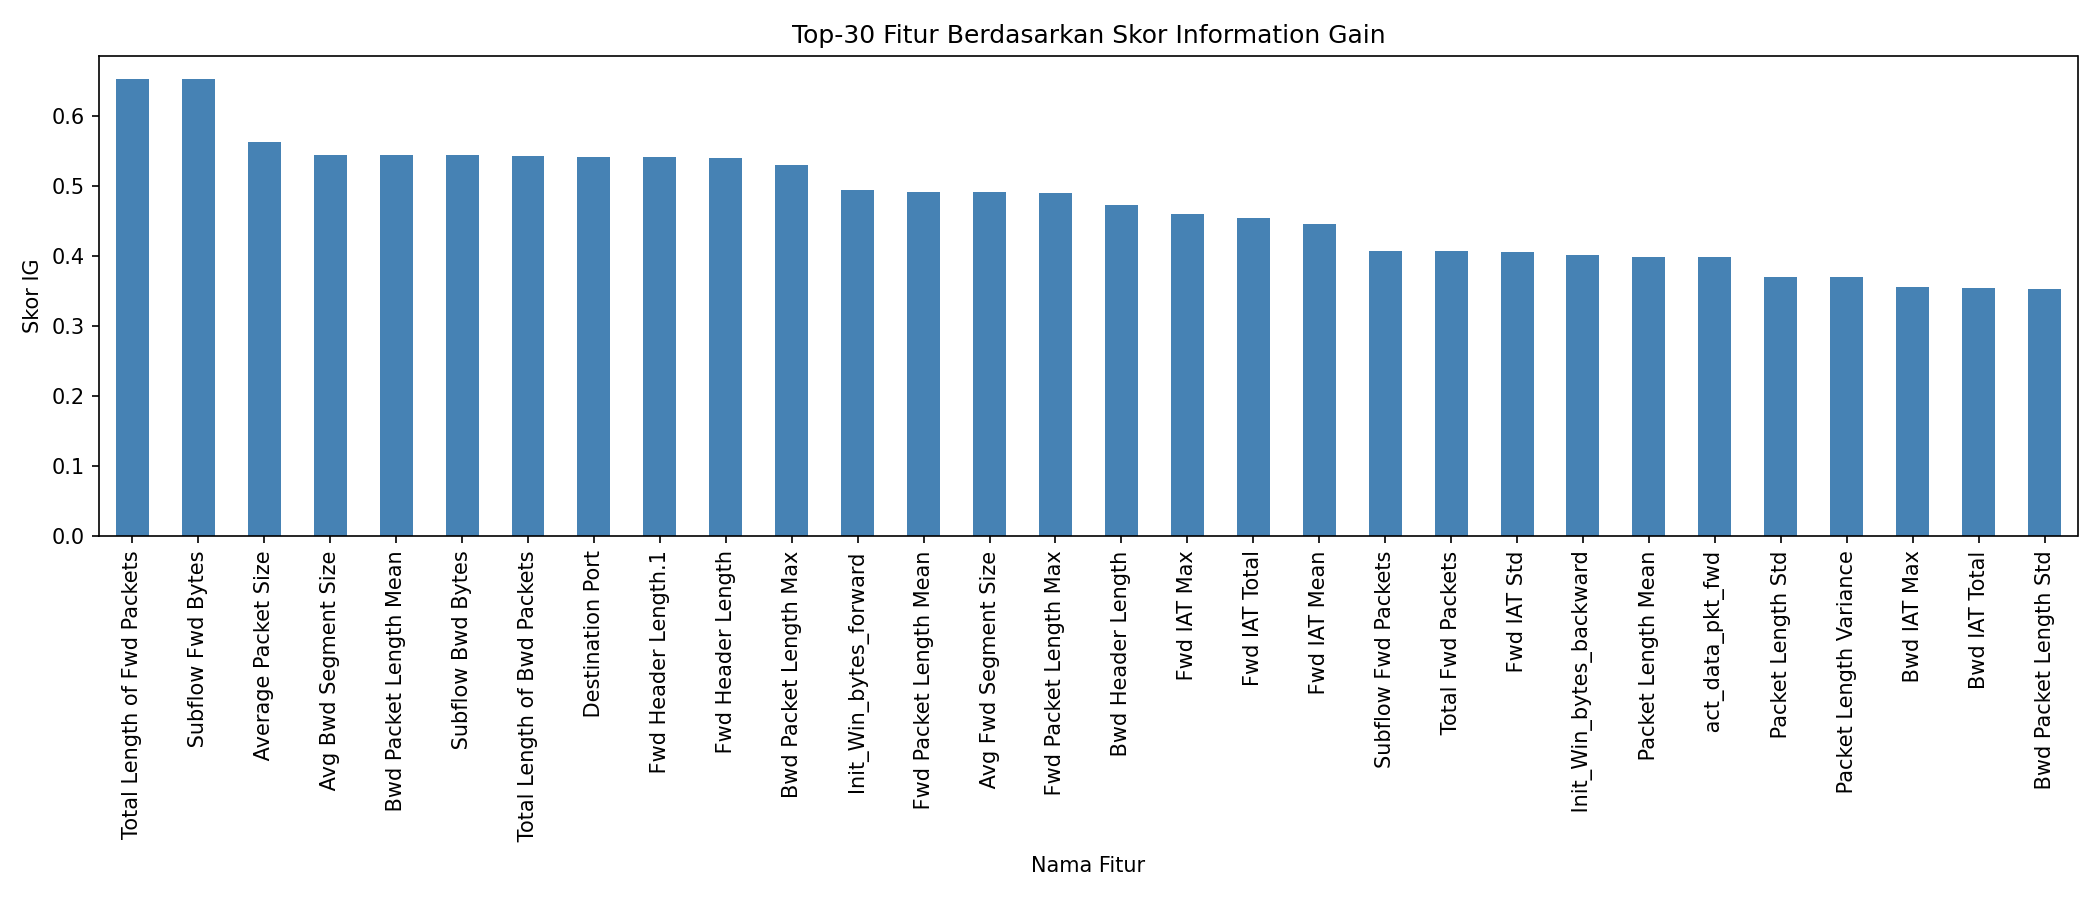
\includegraphics[width=\linewidth]{output/ig_scores_bar.png}
    \vspace{-0.2cm}
    \caption{Top-30 Fitur Berdasarkan Skor \textit{Information Gain}.}
    \vspace{-0.1cm}
    \label{fig:ig}
  \end{minipage}
  \hfill
  \begin{minipage}{0.48\linewidth}
    \centering
    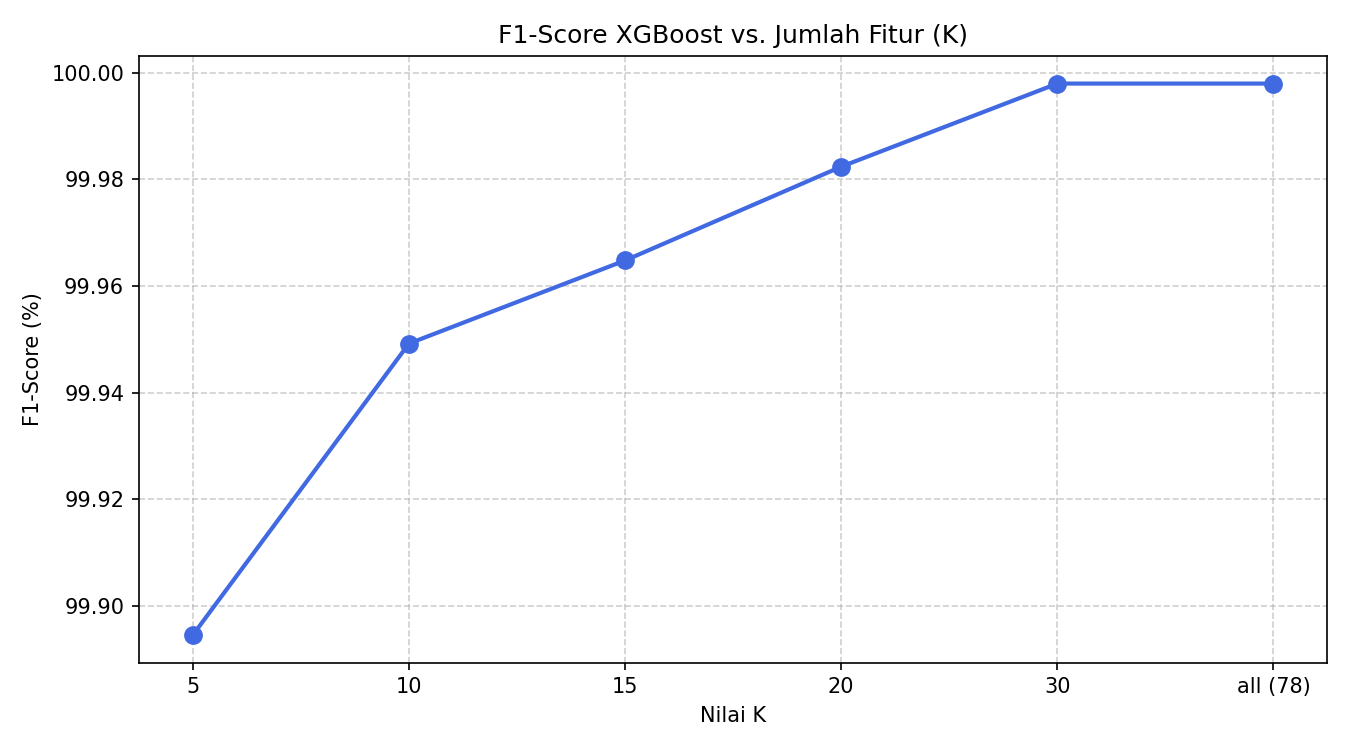
\includegraphics[width=\linewidth]{output/f1_vs_k.png}
    \vspace{-0.2cm}
    \caption{F1-Score XGBoost terhadap Variasi Nilai K.}
    \vspace{-0.1cm}
    \label{fig:f1k}
  \end{minipage}
  \vspace{-0.3cm}
\end{figure}

\subsection{Pengaruh IG terhadap Efisiensi Komputasi}

Dengan mengurangi jumlah fitur dari 78 menjadi K=30, kami berhasil mempercepat waktu pelatihan (\textit{training time})
sebesar \textbf{52,7\%} (dari 9,38\,s menjadi 4,44\,s) tanpa mengurangi akurasi sama sekali. Hal ini sangat penting
karena melatih model dengan sedikit fitur membutuhkan memori dan daya komputasi komputer server yang lebih kecil~\cite{ref_xgboost2016}.

\subsection{Perbandingan XGBoost vs.\ Random Forest}

Tabel~\ref{tab:comparison} menunjukkan perbandingan performa antara XGBoost dan \textit{Random Forest} pada K=30.

\begin{table}[htbp]
\vspace{-0.2cm}
\caption{Perbandingan XGBoost vs.\ Random Forest (K=30)}
\label{tab:comparison}
\centering
\small
\begin{tabular}{lccc}
\toprule
\textbf{Metrik} & \textbf{XGBoost} & \textbf{RF} & \textbf{Selisih} \\
\midrule
Accuracy (\%)        & \textbf{99,9978} & 99,9934 & $+$0,0044 \\
Precision-DDoS (\%)  & \textbf{100,0000} & 99,9961 & $+$0,0039 \\
Recall-DDoS (\%)     & \textbf{99,9961} & 99,9922 & $+$0,0039 \\
F1-Score / macro (\%) & \textbf{99,9977} & 99,9932 & $+$0,0045 \\
AUC-ROC              & \textbf{1,0000} & 1,0000 & 0,0000 \\
FPR (\%)             & \textbf{0,0000} & 0,0051 & $-$0,0051 \\
Training Time (s)    & \textbf{4,44}   & 30,74  & $-26,30$ \\
Inference (ms/flow)  & \textbf{0,0051}  & 0,0084  & $-0,0033$ \\
\bottomrule
\end{tabular}
\end{table}

\begin{figure}[htbp]
  \centering
  \begin{minipage}{0.48\linewidth}
    \centering
    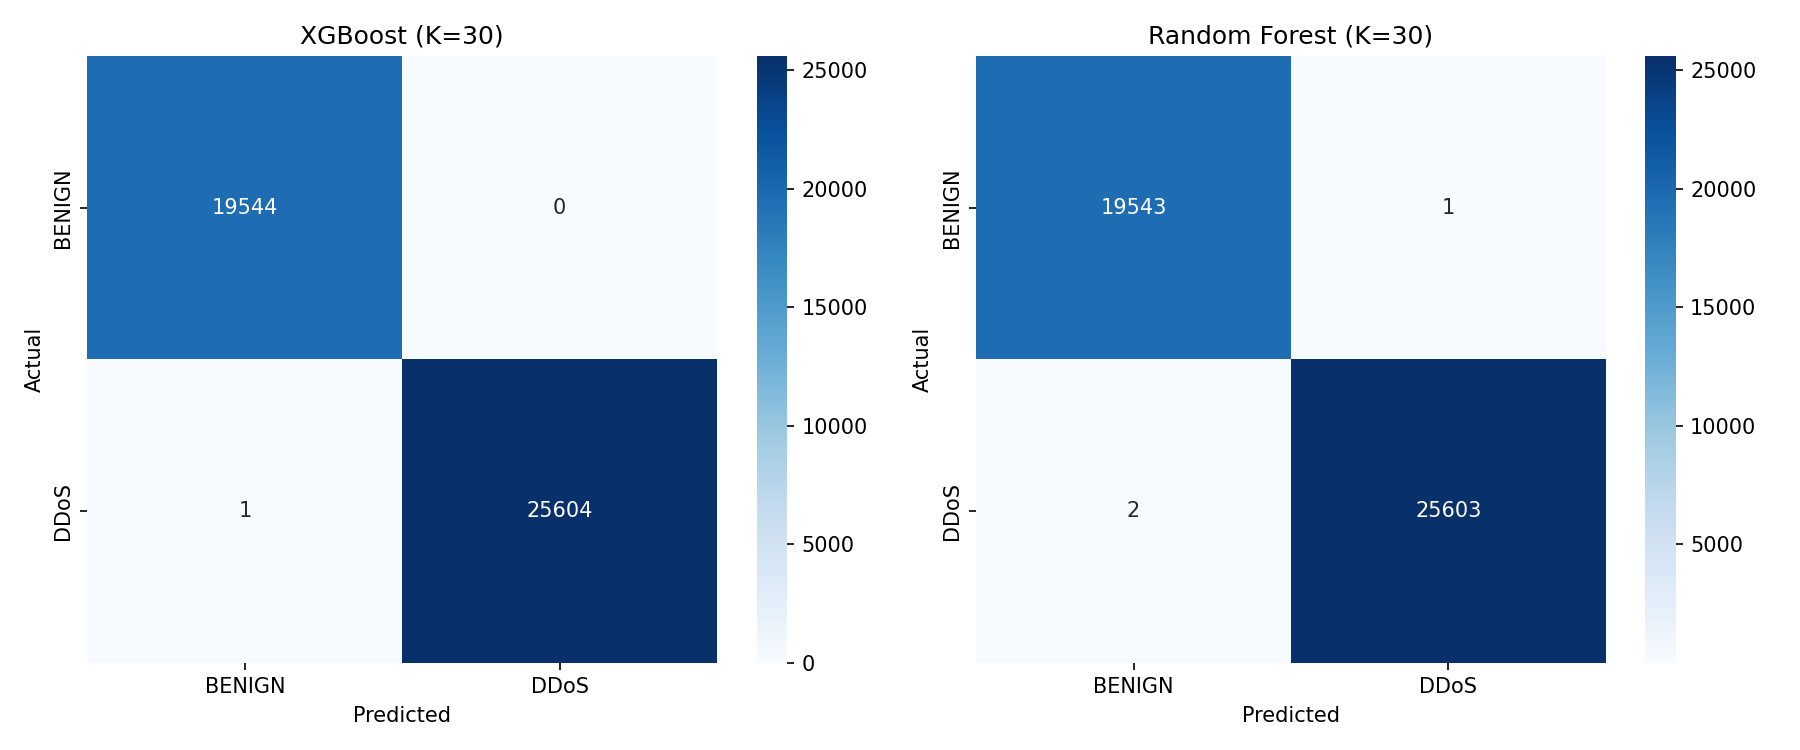
\includegraphics[width=\linewidth]{output/confusion_matrices.png}
    \vspace{-0.2cm}
    \caption{Confusion Matrix XGBoost (kiri) vs.\ RF (kanan) pada K=30.}
    \vspace{-0.1cm}
    \label{fig:cm}
  \end{minipage}
  \hfill
  \begin{minipage}{0.48\linewidth}
    \centering
    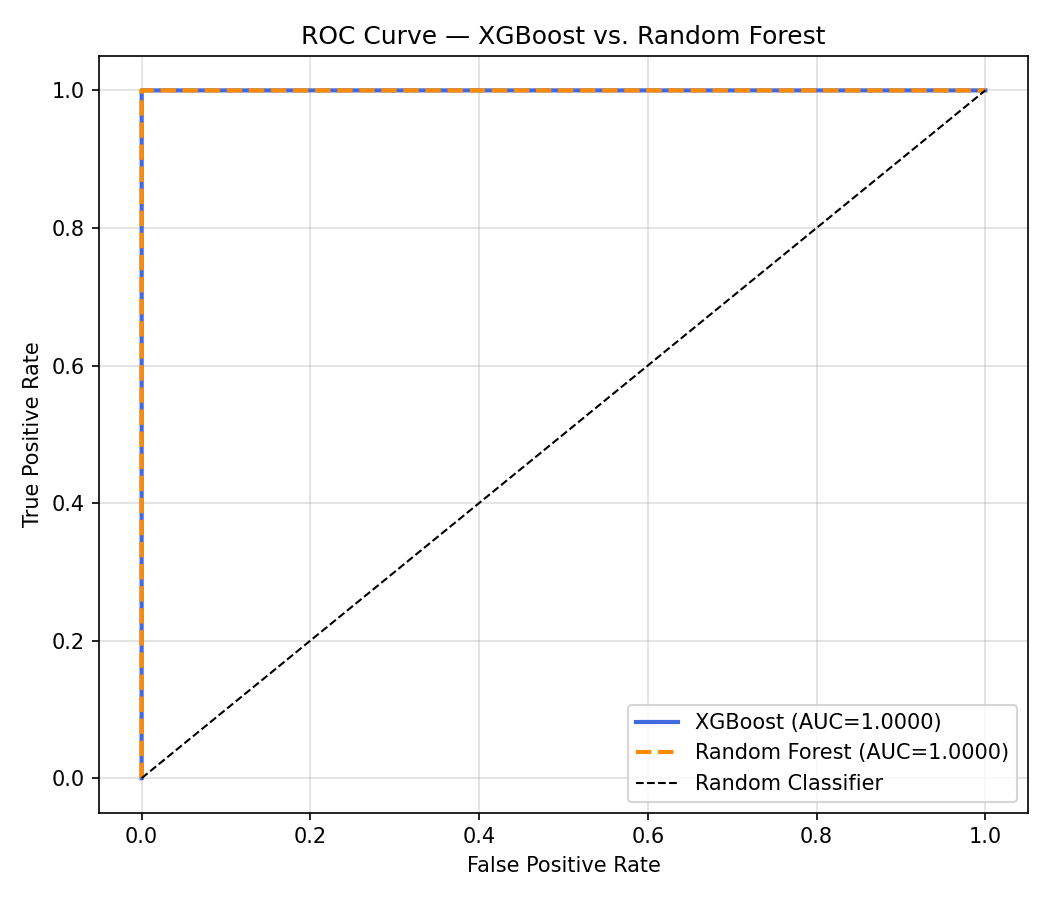
\includegraphics[width=\linewidth]{output/roc_curve.png}
    \vspace{-0.2cm}
    \caption{Kurva ROC XGBoost vs.\ Random Forest (K=30).}
    \vspace{-0.1cm}
    \label{fig:roc}
  \end{minipage}
  \vspace{-0.3cm}
\end{figure}

Dari data tersebut, terlihat bahwa XGBoost sedikit lebih unggul di hampir semua metrik evaluasi, sebagaimana divisualisasikan melalui confusion matrix pada Gambar~\ref{fig:cm} dan kurva ROC pada Gambar~\ref{fig:roc}. XGBoost hanya
salah menebak \textbf{1 sampel} saja dari total 45.149 sampel uji (dengan 1 \textit{False Negative} dan 0 \textit{False Positive}).
Sementara itu, \textit{Random Forest} salah menebak 3 sampel (dengan 2 \textit{False Negative} dan 1 \textit{False Positive}).
Perbedaan performa terbesar ada pada waktu pemrosesan: XGBoost melatih data 6,9$\times$ lebih cepat (4,44\,s vs 30,74\,s)
dan memproses satu flow data 1,6$\times$ lebih cepat (0,0051\,ms vs 0,0084\,ms).

Kami juga menjalankan uji statistik McNemar untuk menguji apakah perbedaan akurasi kedua model ini berbeda secara
signifikan. Hasil uji menghasilkan nilai $\chi^2=0{,}50$ dengan $p=0{,}4795$. Karena nilai $p$ jauh lebih besar dari 0,05,
secara statistik perbedaan tebakan kedua model ini dianggap tidak terlalu berbeda jauh. Keduanya sama-sama sangat akurat,
namun kami memilih XGBoost karena kecepatan komputasinya jauh lebih unggul.

Dibandingkan dengan penelitian terkait yang ditunjukkan pada Tabel~\ref{tab:related_work}, akurasi XGBoost kami
melampaui Thakkar dan Lohiya~\cite{ref_thakkar2020} (99,5\%) dan Kasongo dan Sun~\cite{ref_kasongo2020} (99,2\%),
serta melampaui RF yang dilaporkan Ullah dan Mahmoud~\cite{ref_ullah2020} (98,7\%).

\subsection{Hasil Pengujian DDoShield}

Tabel~\ref{tab:ddoshield} menunjukkan hasil uji performa aplikasi DDoShield saat kami coba mengunggah file \texttt{.pcap}
secara langsung ke server lokal kami.

\begin{table}[htbp]
\vspace{-0.2cm}
\caption{Hasil Pengujian Performa DDoShield}
\label{tab:ddoshield}
\centering
\small
\begin{tabular}{llcc}
\toprule
\textbf{Metrik} & \textbf{Nilai} & \textbf{Satuan} & \textbf{Kondisi} \\
\midrule
Latensi (100 flow)   & 6,08 & ms  & .pcap kecil \\
Latensi (1000 flow)  & 8,89 & ms  & .pcap sedang \\
Latensi (10000 flow) & 56,69 & ms  & .pcap besar \\
Throughput           & 112.512,52 & flow/s & .pcap sedang \\
CPU idle             & 17,1 & \% & Server idle \\
CPU aktif            & 61,0 & \% & 1000 flow \\
Memory idle          & 152,9 & MB & Server idle \\
Memory aktif         & 430,6 & MB & 1000 flow \\
FPR (BENIGN only)    & 0,00 & \% & 100\% normal \\
\bottomrule
\end{tabular}
\end{table}

Aplikasi DDoShield dapat menganalisis file \texttt{.pcap} kecil (100 flow) dengan waktu latensi hanya 6,08\,ms,
pcap sedang (1.000 flow) dalam 8,89\,ms, dan pcap besar (10.000 flow) dalam 56,69\,ms. Kecepatan pemrosesan
inferensi \textit{backend} (\textit{model throughput}) mencapai puncak di angka 112.512,52 flow per detik (angka ini adalah kecepatan prediksi model di memori, tidak termasuk waktu tunggu ekstraksi \textit{parsing} PCAP oleh Scapy). Saat server dalam kondisi diam (\textit{idle}), memori RAM
yang digunakan adalah 152,9\,MB dengan beban CPU 17,1\%. Ketika memproses file dengan 1.000 flow, memori RAM naik
menjadi 430,6\,MB dan beban CPU menjadi 61,0\%. Hasil \textit{False Positive Rate} (FPR) adalah 0,00\%, yang menunjukkan
bahwa aplikasi ini tidak salah mendeteksi data normal sebagai serangan.

Sebagai bukti validitas fungsional (\textit{functional testing}), kami menguji aplikasi ini secara langsung menggunakan sampel berkas \texttt{.pcap} yang memuat jejak serangan jaringan. DDoShield terbukti mampu mengelompokkan paket-paket mentah menjadi aliran terstruktur (\textit{flows}) secara otomatis dan berhasil melabeli aliran serangan secara tepat. Fitur forensik visual \textit{TreeSHAP} pada dasbor DDoShield juga berhasil menyoroti anomali pada fitur \texttt{Flow Packets/s} dan \texttt{Fwd Packet Length} sebagai pemicu vonis DDoS. Temuan ini konsisten dengan hasil analisis manual yang kami lakukan menggunakan Wireshark pada berkas yang sama. Hal ini menjadi bukti bahwa mekanisme \textit{parsing} PCAP dan inferensi XGBoost dalam aplikasi DDoShield berjalan dengan benar dan dapat diandalkan.

% ============================================================
\section{Pembahasan}
\label{sec:diskusi}
% ============================================================

\subsection{Interpretasi Temuan Utama}

Keberhasilan model XGBoost dalam mendeteksi DDoS dengan F1-Score mendekati 100\% dikarenakan cara kerja algoritma
\textit{gradient boosting} yang memperbaiki kesalahan tebakan model sebelumnya di setiap pohon keputusan baru~\cite{ref_xgboost2016}.
Selain itu, teknik regularisasi yang ada pada XGBoost juga sangat membantu mencegah model agar tidak terlalu menghafal
data latih (\textit{overfitting})~\cite{ref_thakkar2020}. Akurasi yang sangat tinggi ini juga dilaporkan oleh peneliti
lain pada dataset CIC-IDS2017~\cite{ref_engelen2021} karena kelas data pada dataset ini memang memiliki pola trafik
yang sangat jelas dibedakan secara statistik.

\subsection{Implikasi Praktis untuk Kampus}

Karena proses pendeteksian XGBoost sangat cepat (0,0051\,ms per flow), aplikasi DDoShield ini dapat diintegrasikan
langsung pada router kampus untuk menganalisis salinan trafik (\textit{port mirroring}) secara berkala. Aplikasi ini juga
dilengkapi dengan REST API sehingga bisa dihubungkan ke sistem pemantauan keamanan lain yang sudah ada di kampus.

\subsection{Validasi dan Keunggulan Dibandingkan Aplikasi Lain}

Untuk memastikan program DDoShield berjalan dengan benar dan hasilnya valid, kami membandingkannya dengan dua aplikasi jaringan yang sudah umum digunakan, yaitu \textbf{Wireshark} dan \textbf{Snort}. Wireshark sering dijadikan standar acuan (\textit{ground truth}) karena mampu menampilkan isi paket jaringan secara langsung. Namun, menganalisis ratusan ribu paket DDoS di Wireshark secara manual tentu membutuhkan waktu lama dan rawan terjadi kesalahan. Sementara itu, Snort adalah aplikasi pendeteksi penyusupan (IDS) yang cepat, tetapi karena berbasis aturan statis (\textit{signature-based}), ia sering kesulitan mendeteksi serangan tipe baru (\textit{zero-day}) yang belum ada aturannya.

\begin{table*}[t]
\vspace{-0.2cm}
\caption{Perbandingan Validasi DDoShield dengan Aplikasi Jaringan Umum}
\label{tab:comparison_tools}
\centering
\small
\setlength{\tabcolsep}{6pt}
\begin{tabular}{p{3.5cm}p{4cm}p{4cm}p{4cm}}
\toprule
\textbf{Kriteria} & \textbf{DDoShield (Kami)} & \textbf{Wireshark} & \textbf{Snort} \\
\midrule
Metode Analisis & Machine Learning & Inspeksi Manual & Aturan Statis (\textit{Signature}) \\
Validitas Hasil & Sangat Tinggi (Berdasarkan Dataset) & Standar Acuan Utama & Bergantung \textit{Update} Aturan \\
Deteksi Serangan Baru & Bisa (Melihat Pola Anomali) & Bisa (Tergantung Analis) & Tidak Bisa \\
Kecepatan Deteksi & Sangat Cepat (0,0051 ms/flow) & Lambat (Manual) & Cepat (Otomatis) \\
Cara Analisis (Forensik) & Grafik Visual (\textit{TreeSHAP}) & Baca Kode \textit{Hex/Bytes} & Baca Teks Peringatan (\textit{Alert}) \\
\bottomrule
\end{tabular}
\end{table*}

DDoShield hadir untuk menutupi kekurangan kedua aplikasi tersebut. Seperti yang ditunjukkan pada Tabel~\ref{tab:comparison_tools}, DDoShield memberikan akurasi pendeteksian yang valid dengan waktu proses yang jauh lebih efisien dibandingkan analisis manual Wireshark. Berbeda dengan Snort yang kaku pada aturan, model XGBoost pada DDoShield berpotensi mengenali varian serangan yang belum memiliki \textit{signature} karena klasifikasinya berbasis pola statistik aliran (\textit{flow statistics}), bukan pencocokan teks paket. Meskipun demikian, kemampuan ini belum diuji secara eksplisit pada serangan \textit{zero-day} dalam penelitian ini. Selain itu, untuk keperluan forensik, DDoShield menyediakan grafik \textit{TreeSHAP} yang langsung menampilkan fitur penyebab serangan. Hal ini memudahkan pengguna untuk melakukan evaluasi tanpa harus menganalisis kode \textit{byte heksadesimal} paket yang rumit seperti di Wireshark. Dengan demikian, program ini tidak hanya akurat secara komputasi, tetapi juga mudah dan praktis digunakan.



\subsection{Keterbatasan}

Adapun beberapa keterbatasan ruang lingkup dalam penelitian ini meliputi: (1)~penggunaan dataset standar CIC-IDS2017 sebagai representasi trafik simulasi~\cite{ref_engelen2021}; (2)~meskipun DDoShield mendukung mode \textit{Live Sniffing}, evaluasi performa pada penelitian ini difokuskan pada mode analisis berkas \texttt{.pcap} rekaman (\textit{offline capture}); (3)~uji coba performa aplikasi yang dibatasi pada satu komputer server lokal; dan (4)~model belum dievaluasi terhadap jenis serangan siber terbaru yang menggunakan teknik manipulasi data (\textit{adversarial attacks}).

\subsection{Arah Penelitian Mendatang}

Untuk penelitian selanjutnya, kami berencana untuk: (1)~mengumpulkan data trafik langsung dari jaringan kampus kami;
(2)~mengembangkan sistem deteksi \textit{real-time} dari trafik jaringan yang mengalir langsung (\textit{live capture});
(3)~menguji ketahanan model terhadap serangan yang dimanipulasi; dan (4)~mencoba metode pembaruan model secara otomatis
agar tetap akurat seiring berjalannya waktu (\textit{continual learning}).

% ============================================================
\section{Kesimpulan}
\label{sec:kesimpulan}
% ============================================================

Dalam penelitian ini, kami telah mengembangkan dan mengevaluasi sistem deteksi DDoS berbasis XGBoost dengan seleksi fitur
\textit{Information Gain}. Kami juga membuat prototipe aplikasi web bernama DDoShield untuk membantu mendeteksi serangan
di jaringan kampus secara lebih mudah.

Model XGBoost dengan $K=30$ fitur terbaik berhasil mencapai \textit{F1-Score} sebesar 99,9977\% dan nilai AUC-ROC sebesar 1,0000.
Dari 45.149 data uji, model kami hanya salah menebak 1 data saja, sedikit lebih baik dibandingkan dengan \textit{Random Forest}
(99,9932\%). Metode seleksi fitur IG terbukti sangat membantu karena dapat memotong waktu pelatihan sebesar 52,7\% tanpa menurunkan
akurasi. Uji McNemar menunjukkan akurasi kedua model tidak berbeda secara signifikan secara statistik ($p=0{,}4795$), namun XGBoost
jauh lebih cepat dalam melatih data (6,9$\times$ lebih cepat) dan memproses flow (1,6$\times$ lebih cepat).

Hasil ini membuktikan bahwa kombinasi XGBoost dan seleksi fitur IG sangat cocok digunakan untuk mendeteksi DDoS di kampus yang
memiliki keterbatasan sumber daya komputer. Di masa depan, kami berharap bisa menguji sistem ini menggunakan trafik kampus nyata
secara langsung.

% ── UCAPAN TERIMA KASIH ──────────────────────────────────────
\section*{Ucapan Terima Kasih}

Para penulis mengucapkan terima kasih kepada Program Studi Rekayasa Keamanan Siber, Politeknik Siber dan Sandi Negara, atas
dukungan akademik selama penelitian ini. Terima kasih juga kepada \textit{Canadian Institute for Cybersecurity}, Universitas New Brunswick, atas ketersediaan dataset CIC-IDS2017 yang digunakan dalam penelitian ini.

% ── DAFTAR PUSTAKA ───────────────────────────────────────────
\vspace{-0.2cm}
\balance
\bibliographystyle{IEEEtran}
\scriptsize
\bibliography{references}

\end{document}
